\documentclass{beamer}

% choose options for [] as required from the list
% in the Reference Guide

\usepackage{mathptmx}       % selects Times Roman as basic font
\usepackage{helvet}         % selects Helvetica as sans-serif font
\usepackage{courier}        % selects Courier as typewriter font
\usepackage{type1cm}        % activate if the above 3 fonts are
                            % not available on your system
%
\usepackage{makeidx}         % allows index generation
\usepackage{graphicx}        % standard LaTeX graphics tool
                             % when including figure files
\usepackage{multicol}        % used for the two-column index
\usepackage[bottom]{footmisc}% places footnotes at page bottom

\usepackage{amsmath}
\usepackage{amssymb}
\usepackage{txfonts}
\usepackage{algorithm2e}
\usepackage{nicefrac}
\usepackage{multimedia}
\usepackage{float}
\usepackage{ifthen}
\usepackage{fancybox}
\usepackage{tikz}

\newcommand\bref[1]{{\scriptsize[#1]}}
\newcommand\bpic[3]{%
  \color{ethbluedarkfg}%
  \ifthenelse{\equal{#3}{}}{%
    \begin{pgfpictureboxed}{0cm}{0cm}{#1}{#2}%
      \pgfbox[left,bottom]{\tiny\;No image}%
    \end{pgfpictureboxed}}{%
    \includegraphics[width=#1,height=#2]{#3}}%
}
\newcommand\alertbox[1]{\fcolorbox{ethgraydarkfg}{ethbluelightbg!50!white}{#1}}

\usetheme{eth}

%%%%%%%%%%%%%%%%%%%%%%%%%%%%%%%%%%%%%%%%%%%%%%%%%%%%%%%%%%%%%%%%%%%%%%%%%%%%%%%%%%%%%%%%%

\begin{document}

\title{Bayesian Online Learning of Driving Behaviors}
\author[J\'er\^ome Maye]{
J\'er\^ome Maye$^*$, Rudolph Triebel$^*$, Luciano Spinello$^+$, Roland
  Siegwart$^*$
}
\institute{
* Autonomous Systems Lab, ETH Zurich, Switzerland \\
+ Social Robotics Lab, University of Freiburg, Germany \\
}
\date{May 11, 2011}

\maketitleframe

\section{Introduction}

\subsection{Motivation}
\begin{frame}[t]
  \frametitle{Motivation}
  \begin{columns}[c]
    \begin{column}{5cm}
      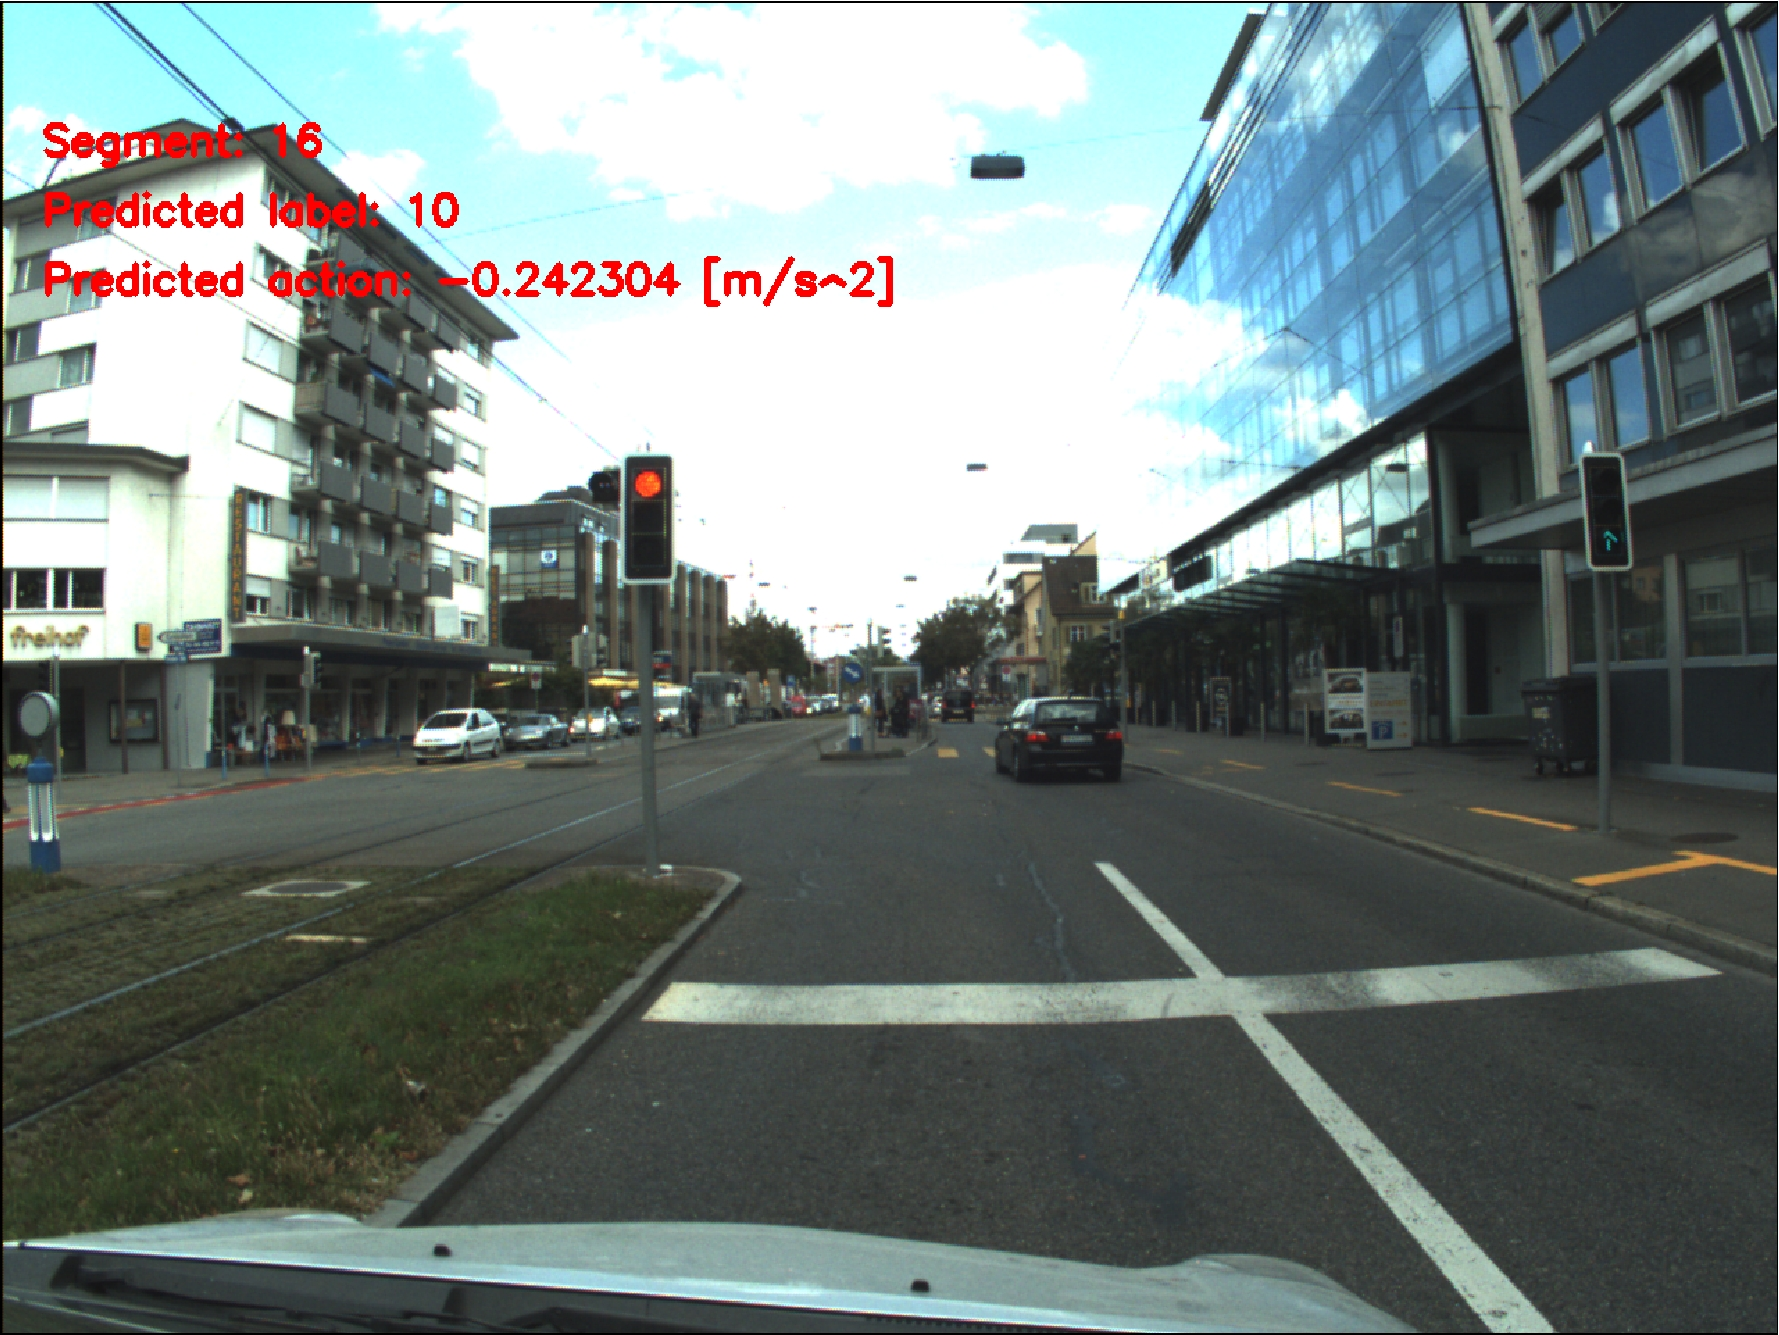
\includegraphics[scale=0.13]{figures/finalResult}
    \end{column}
    \begin{column}{5cm}
      \begin{itemize}
        \item Understanding complex traffic situations
        \item Learning and predicting human driving behaviors from visual scenes
        \item Online, unsupervised, and incremental learning
        \item Driver assistance systems and autonomous navigation applications
      \end{itemize}
    \end{column}
  \end{columns}
\end{frame}

\subsection{Problem Description and Approach}
\begin{frame}[t]
  \frametitle{Problem Description and Approach}
  \begin{itemize}
    \item Learn the relationship between IMU and monocular camera
    \item Assumption: IMU data can be decomposed into chunks corresponding
      to driving behaviors (braking, turning, \dots)
    \item Image categorization into the segmented motion chunks
    \item Driving behavior model for each scene category
    \item Incremental and generative models
  \end{itemize}
  \begin{center}
    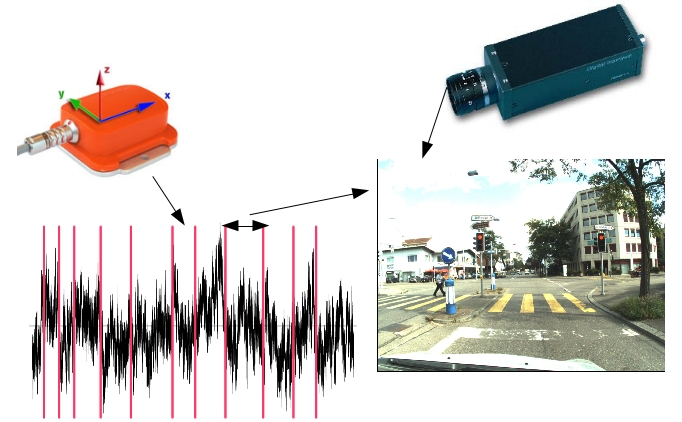
\includegraphics[scale=0.2]{figures/overview}
  \end{center}
\end{frame}

\subsection{Probabilistic Formulation}
\begin{frame}[t]
  \frametitle{Probabilistic Formulation}
  \begin{itemize}
    \item Observable random variables:
      \begin{itemize}
        \item $\mathbf{z}_t$: IMU data at time $t$
        \item $\mathbf{c}_t$: camera data at time $t$
      \end{itemize}
    \item Latent random variables:
      \begin{itemize}
        \item $r_t$: motion segment length at time $t$
        \item $l_t$: visual scene label at time $t$
        \item $\mathbf{a}_t$: action prediction at time $t$
      \end{itemize}
    \item Estimation of $p(r_t,l_t,\mathbf{a}_t\mid\mathbf{z}_{1:t},
      \mathbf{c}_{1:t})=$\\$p(r_t\mid\mathbf{z}_{1:t})$
      $p(l_t\mid r_t,
      \mathbf{c}_{1:t})$
      $p(\mathbf{a}_t\mid r_t,l_t,
      \mathbf{z}_{1:t})$
  \end{itemize}
\end{frame}

\begin{frame}[t]
  \frametitle{Probabilistic Formulation}
  \begin{itemize}
    \item Observable random variables:
      \begin{itemize}
        \item $\mathbf{z}_t$: IMU data at time $t$
        \item $\mathbf{c}_t$: camera data at time $t$
      \end{itemize}
    \item Latent random variables:
      \begin{itemize}
        \item $r_t$: motion segment length at time $t$
        \item $l_t$: visual scene label at time $t$
        \item $\mathbf{a}_t$: action prediction at time $t$
      \end{itemize}
    \item Estimation of $p(r_t,l_t,\mathbf{a}_t\mid\mathbf{z}_{1:t},
      \mathbf{c}_{1:t})=$\\\alertbox{$p(r_t\mid\mathbf{z}_{1:t})$}
      $p(l_t\mid r_t,
      \mathbf{c}_{1:t})$
      $p(\mathbf{a}_t\mid r_t,l_t,
      \mathbf{z}_{1:t})$
  \end{itemize}
\end{frame}

\section{Motion Segmentation}
\subsection{Changepoint Detection}
\begin{frame}[t]
  \frametitle{Changepoint Detection \tt{[Fearnhead, 2007]}}
  \begin{columns}[c]
    \begin{column}{5cm}
      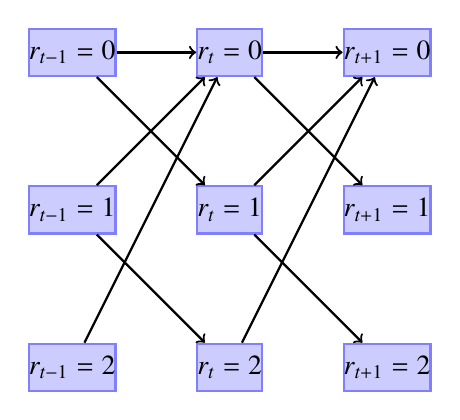
\begin{tikzpicture}[scale=0.5]
        \tikzstyle{every node} = [rectangle,draw=blue!50,fill=blue!20,thick,
          inner sep=0pt,minimum size=6mm]
        \node (a) at (-4, 4) {$r_{t-1}=0$};
        \node (b) at (-4, 0) {$r_{t-1}=1$};
        \node (c) at (-4, -4) {$r_{t-1}=2$};
        \node (d) at (0, 4) {$r_t=0$};
        \node (e) at (0, 0) {$r_t=1$};
        \node (f) at (0, -4) {$r_t=2$};
        \node (g) at (4, 4) {$r_{t+1}=0$};
        \node (h) at (4, 0) {$r_{t+1}=1$};
        \node (i) at (4, -4) {$r_{t+1}=2$};
        \draw [->,thick] (a) -- (d);
        \draw [->,thick] (a) -- (e);
        \draw [->,thick] (b) -- (d);
        \draw [->,thick] (b) -- (f);
        \draw [->,thick] (c) -- (d);
        \draw [->,thick] (d) -- (h);
        \draw [->,thick] (d) -- (g);
        \draw [->,thick] (e) -- (i);
        \draw [->,thick] (e) -- (g);
        \draw [->,thick] (f) -- (g);
      \end{tikzpicture}
    \end{column}
    \begin{column}{5cm}
      \begin{itemize}
        \item CP = change in generative parameters
        \item Inference on \alertbox{$p(r_t\mid\mathbf{z}_{1:t})$}
        \item Recursive message-passing algorithm
        \item Transition probability and predictive distribution
        \item Particle filter for constant time update
      \end{itemize}
    \end{column}
  \end{columns}
\end{frame}

\subsection{IMU Data Segmentation}
\begin{frame}[t]
  \frametitle{IMU Data Segmentation}
  \begin{itemize}
    \item IMU data $\mathbf{z}_t\sim\mathcal{N}(\mathbf{z}_t\mid
      \boldsymbol{\mu}_i,\boldsymbol{\Sigma}_i)$, $i=1:N$ motion segments
    \item Normal-Wishart conjugate prior for estimating $\boldsymbol{\mu}_t,
      \boldsymbol{\Sigma}_t$ using $\mathbf{z}_t$
    \item Predictive distribution approximated with Student-$t$
    \item Transition probability modeled as a hazard function
  \end{itemize}
  \begin{center}
    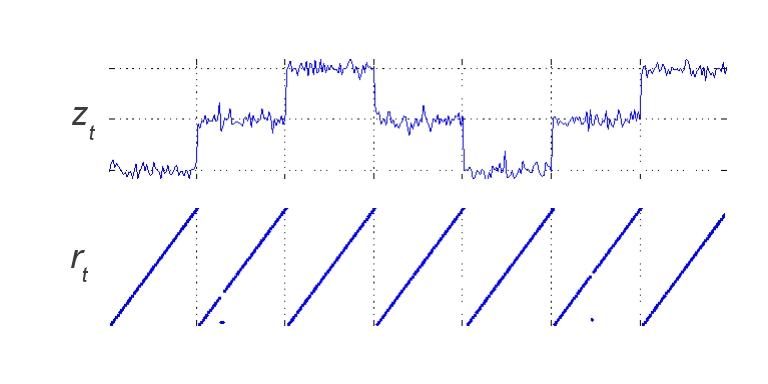
\includegraphics[scale=0.3]{figures/cpExample}
  \end{center}
\end{frame}

\begin{frame}[t]
  \frametitle{Probabilistic Formulation}
  \begin{itemize}
    \item Observable random variables:
      \begin{itemize}
        \item $\mathbf{z}_t$: IMU data at time $t$
        \item $\mathbf{c}_t$: camera data at time $t$
      \end{itemize}
    \item Latent random variables:
      \begin{itemize}
        \item $r_t$: motion segment length at time $t$
        \item $l_t$: visual scene label at time $t$
        \item $\mathbf{a}_t$: action prediction at time $t$
      \end{itemize}
    \item Estimation of $p(r_t,l_t,\mathbf{a}_t\mid\mathbf{z}_{1:t},
      \mathbf{c}_{1:t})=$\\$p(r_t\mid\mathbf{z}_{1:t})$
      \alertbox{$p(l_t\mid r_t,
      \mathbf{c}_{1:t})$}
      $p(\mathbf{a}_t\mid r_t,l_t,
      \mathbf{z}_{1:t})$
  \end{itemize}
\end{frame}

\section{Visual Scene Categorization}
\subsection{Image Processing}
\begin{frame}[t]
  \frametitle{Image Processing - Bag of Words}
  \begin{columns}[c]
    \begin{column}{5cm}
      \begin{itemize}
        \item SIFT keypoints and descriptors
        \item Dictionary generation with K-means algorithm
        \item Assign each descriptor to the closest word
        \item Input data $\mathbf{c}_t$ as a vector of word counts (BoW)
      \end{itemize}
    \end{column}
    \begin{column}{5cm}
      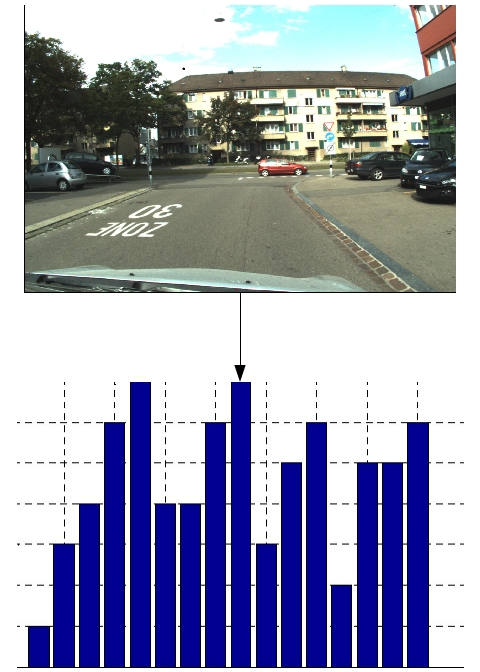
\includegraphics[scale=0.22]{figures/bow}
    \end{column}
  \end{columns}
\end{frame}

\subsection{Image Categorization}
\begin{frame}[t]
  \frametitle{Image Categorization}
  \begin{itemize}
    \item Inference on \alertbox
      {$p(l_t\mid r_t,\mathbf{c}_{1:t})$} $\propto$
      $p(\mathbf{c}_t\mid l_t,r_t,\mathbf{c}_{t-1})p(l_t\mid r_t,
      \mathbf{c}_{1:t-1})$
    \item $p(\mathbf{c}_t\mid l_t,r_t,\mathbf{c}_{t-1})\sim$ Dirichlet Compound
      Multinomial distribution
    \item Dirichlet hyperparameter $\boldsymbol{\alpha}_i$ for each value of
      $l_t$
    \item Bayesian update of the $\boldsymbol{\alpha}_i$ with $\mathbf{c}_t$
    \item Decision for new models with Bayes factor
  \end{itemize}
  \begin{center}
    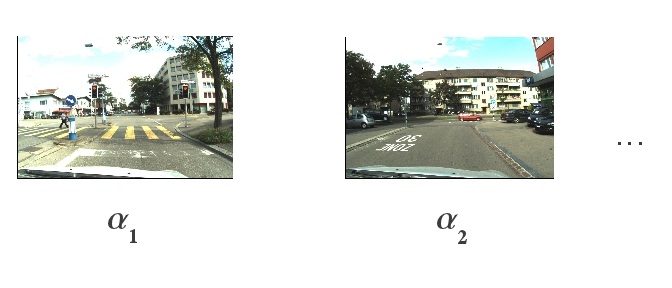
\includegraphics[scale=0.35]{figures/label}
  \end{center}
\end{frame}

\begin{frame}[t]
  \frametitle{Probabilistic Formulation}
  \begin{itemize}
    \item Observable random variables:
      \begin{itemize}
        \item $\mathbf{z}_t$: IMU data at time $t$
        \item $\mathbf{c}_t$: camera data at time $t$
      \end{itemize}
    \item Latent random variables:
      \begin{itemize}
        \item $r_t$: motion segment length at time $t$
        \item $l_t$: visual scene label at time $t$
        \item $\mathbf{a}_t$: action prediction at time $t$
      \end{itemize}
    \item Estimation of $p(r_t,l_t,\mathbf{a}_t\mid\mathbf{z}_{1:t},
      \mathbf{c}_{1:t})=$\\$p(r_t\mid\mathbf{z}_{1:t})$
      $p(l_t\mid r_t,
      \mathbf{c}_{1:t})$
      \alertbox{$p(\mathbf{a}_t\mid r_t,l_t,
      \mathbf{z}_{1:t})$}
  \end{itemize}
\end{frame}

\section{Actions Learning and Prediction}
\begin{frame}[t]
  \frametitle{Action Learning and Prediction}
  \begin{itemize}
    \item Inference on \alertbox
      {$p(\mathbf{a_t}\mid r_t, l_t,\mathbf{z}_{1:t})$}$\sim$ Gaussian Mixture
      Model (GMM)
    \item Model different potential actions in a visual scene
    \item One GMM for each value of $l_t$
    \item Online learning of GMM parameters
  \end{itemize}
  \begin{center}
    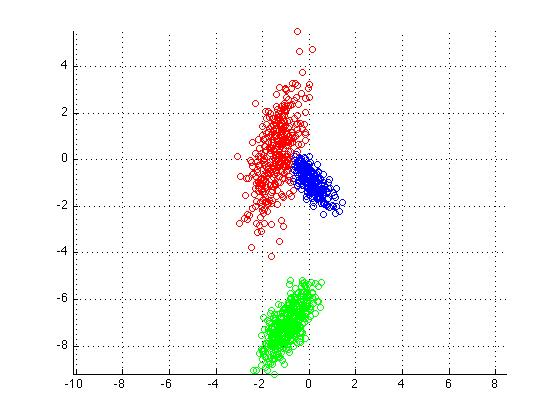
\includegraphics[scale=0.24]{figures/gmm}
  \end{center}
\end{frame}

\section{Experiments}
\subsection{Simulated Data}
\begin{frame}[t]
  \frametitle{Experiments - Simulated Data}
  \begin{center}
    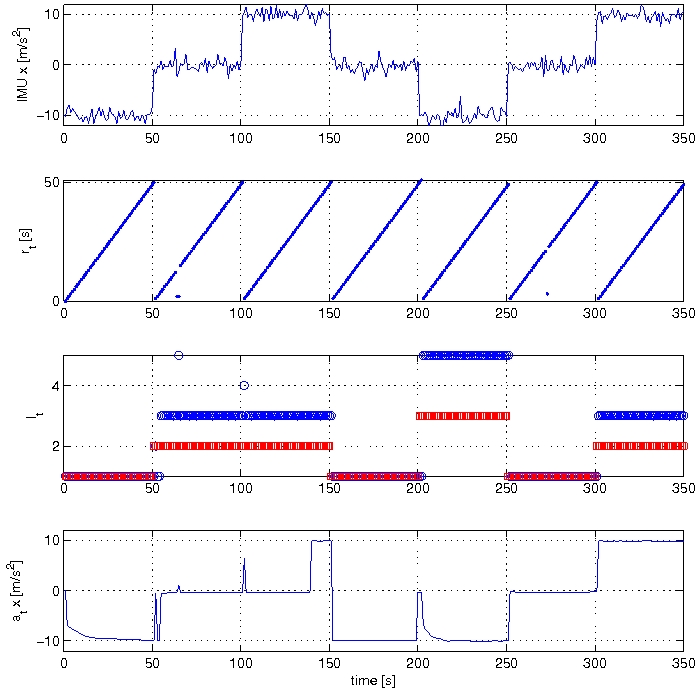
\includegraphics[scale=0.33]{figures/simResult}
  \end{center}
\end{frame}

\subsection{Motion Segmentation}
\begin{frame}[t]
  \frametitle{Experiments - Motion Segmentation}
  \begin{columns}[c]
    \begin{column}{5cm}
      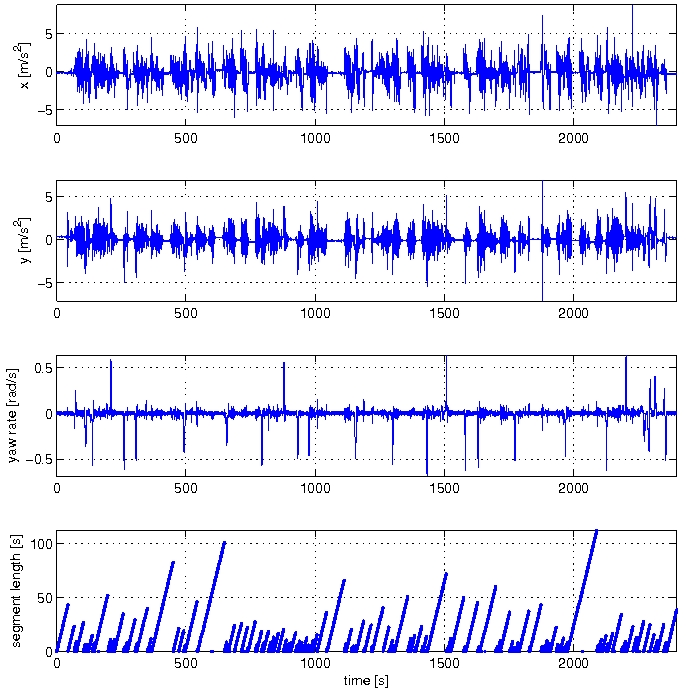
\includegraphics[scale=0.3]{figures/cpResult}
    \end{column}
    \begin{column}{5cm}
      \begin{itemize}
        \item 40 minutes run around the city (3 loops)
        \item Traffic lights, pedestrian crossings, stop and yield signs, \dots
        \item Manual labeling for ground truth
        \item $92\%$ accuracy
      \end{itemize}
    \end{column}
  \end{columns}
\end{frame}

\subsection{Labeling and Motion Prediction}
\begin{frame}[t]
  \frametitle{Experiments - Labeling and Motion Prediction}
  \begin{itemize}
    \item Supervised setting:
      \begin{itemize}
        \item Traffic lights: $93\%$ accuracy
        \item Yield signs: $99\%$ accuracy
        \item Pedestrian crossings: $91\%$ accuracy
      \end{itemize}
    \item Unsupervised setting:
      \begin{itemize}
        \item Hard to evaluate quantitatively
        \item Label re-association during the 3 loops
        \item Similar scenes receive the same label
      \end{itemize}
    \item Motion prediction:
      \begin{itemize}
        \item Evaluated qualitatively by visual inspection
        \item Predicted actions correspond to expected behavior
      \end{itemize}
  \end{itemize}
\end{frame}

\section{Conclusions and Prospection}
\begin{frame}[t]
  \frametitle{Conclusions and Prospection}
  \begin{itemize}
    \item Online, unsupervised, and incremental understanding of complex traffic
      scenes
    \item Learning relationship between IMU and camera data
    \item Ability to start from scratch and perform continuous learning
  \end{itemize}
  \begin{itemize}
    \item Further possible research on image and behaviors modeling
    \item Implementation and testing on a car
  \end{itemize}
\end{frame}

\begin{frame}[t]
  \frametitle{Questions}
  \begin{itemize}
    \item Thank you for your attention!
  \end{itemize}
\end{frame}

\end{document}
